\appendix



\begin{deluxetable}{ccrrrrrrrrcrl}
\tabletypesize{\scriptsize}

\tablecaption{Elevation and Azimuth of the Sun for 02/26/2012 \cite{sunbb}}
\tablewidth{0pt}
\tablehead{
\colhead{Eastern Time } & \colhead{Elevation} & \colhead{Azimuth (E of N)} 
}
\startdata                                                                                 
10:50 &      37.4   &    155.2\\
11:00  &     38.1   &    159.3\\
11:10   &    38.7   &    162.3\\
11:20   &    39.2   &    165.4\\
11:30 &      39.7   &    168.6\\
11:40  &     40.0   &    171.8\\
11:50   &    40.2   &    175.0\\
12:00   &    40.3   &    178.2\\
12:10   &    40.3    &   181.5\\
12:20  &     40.2    &   184.7\\
\enddata
\tablecomments{The altitude and azimuth of the Sun for the day of the observations, 02/26/2012,  at Stony Brook University, NY,W 73 08, N40 56.}
\label{a-sun}
\end{deluxetable}


\begin{deluxetable}{ccrrrrrrrrcrl}
\tabletypesize{\scriptsize}

\tablecaption{Measured and Calculated Baseline Lengths }
\tablewidth{0pt}
\tablehead{
\colhead{Baseline Measured  } & \colhead{Length (m)} & \colhead{Baseline Satellite } & \colhead{ Length (m)} & \colhead{Baseline Sun }& \colhead{Length (m)}}
\startdata                                                                                 
$B^{meas}_{1}$ & $0.60 \pm 0.05$ & $B^{sat}_{1}$& $1.40 \pm 1.16$ & $B^{sun}_{1}$  & $1.01 \pm 1.16$\\
$B^{meas}_{2}$ & $0.76 \pm 0.05 $ & $B^{sat}_{2}$& $1.62 \pm 1.16$ & $B^{sun}_{2}$ & $1.33 \pm 1.16$\\
$B^{meas}_{3}$ & $0.92 \pm 0.05$& $B^{sat}_{3}$& $1.85 \pm 1.16$ & $B^{sun}_{3}$ & $1.64 \pm 1.16$\\
$B^{meas}_{4}$&  $1.08 \pm 0.05$ & $B^{sat}_{4}$& $2.16 \pm 1.16$ & $B^{sun}_{4}$ & $2.02 \pm 1.16$\\
$B^{meas}_{5}$ & $1.24 \pm  0.05$ &$B^{sat}_{5}$& $2.30 \pm 1.16$  & $B^{sun}_{5}$ & $2.13 \pm 1.16$ \\
\enddata
\tablecomments{The first values are the baseline lengths  measured from the left border of the left mirror to the right border of the right mirror. The accurate length measurement should have be done from the middle of the both mirror. In the final calculations we use the baseline lengths calculated from the analysis, \ie the second and third values of the table. The measured  values are included for completeness only.  Although the uncertainty for them (which are based on the half of the minimum size of the ruler) are smaller than for the calculated values, it does not imply that the first values are more precise.}
\label{baselines}
\end{deluxetable}





\begin{deluxetable}{ccrrrrrrrrcrl}
\tabletypesize{\scriptsize}

\tablecaption{Time and Angle Range for the Interferometer Measurements for the Sun}
\tablewidth{0pt}
\tablehead{
\colhead{Baseline Label in the Analysis } & \colhead{Filename} & \colhead{Angle Range  in Degrees} & \colhead{Eastern Time} & \colhead{Sun's Azimuth}}
\startdata                                                                                 
$B^{sun}_{1}$ &  SUN1&-10,10 &1050&155.2\\
$B^{sun}_{2}$&	SUN2 &-15,5&1105&	162.3\\
$B^{sun}_{3}$&	SUN3&	-15,5&1115	&165\\
$B^{sun}_{4}$&	SUN41&	-15,5&1118	&165.4\\
$B^{sun}_{4}$&	SUN42&	-10,10	&1120	&165.4\\
$B^{sun}_{5}$&	SUN5&	-10,10	&1123	&165.4\\
\enddata
\tablecomments{Data from the log book. The file SUN42 is the same data than SUN41 so it was not used in the analysis. We refer to SUN4 instead than SUN41.}
\label{sun}
\end{deluxetable}


\begin{deluxetable}{ccrrrrrrrrcrl}
\tabletypesize{\scriptsize}

\tablecaption{Time and Angle Range for the Interferometer Measurements for the Satellite}
\tablewidth{0pt}
\tablehead{
\colhead{Baseline Label in the Analysis } & \colhead{Filename} & \colhead{Angle Range in Degrees} & \colhead{Eastern Time} & \colhead{Satellite's Azimuth}}
\startdata   
$B^{sun}_{1}$& SAT1	&	20,30	&	1219  & \\
$B^{sun}_{2}$& SAT2	&	20,30	&	1217
 &  \\
$B^{sun}_{3}$& SAT3	&	20,30	&	1215
 & \\
$B^{sun}_{4}$& 	SAT4	&	20,20	&	1213
 &   \\
$B^{sun}_{5}$& SAT5	&	20,30	&	1205
&   \\
\enddata
\tablecomments{Data from the log book.}
\label{sat}
\end{deluxetable}


 \begin{figure}[htb]
\begin{center}
 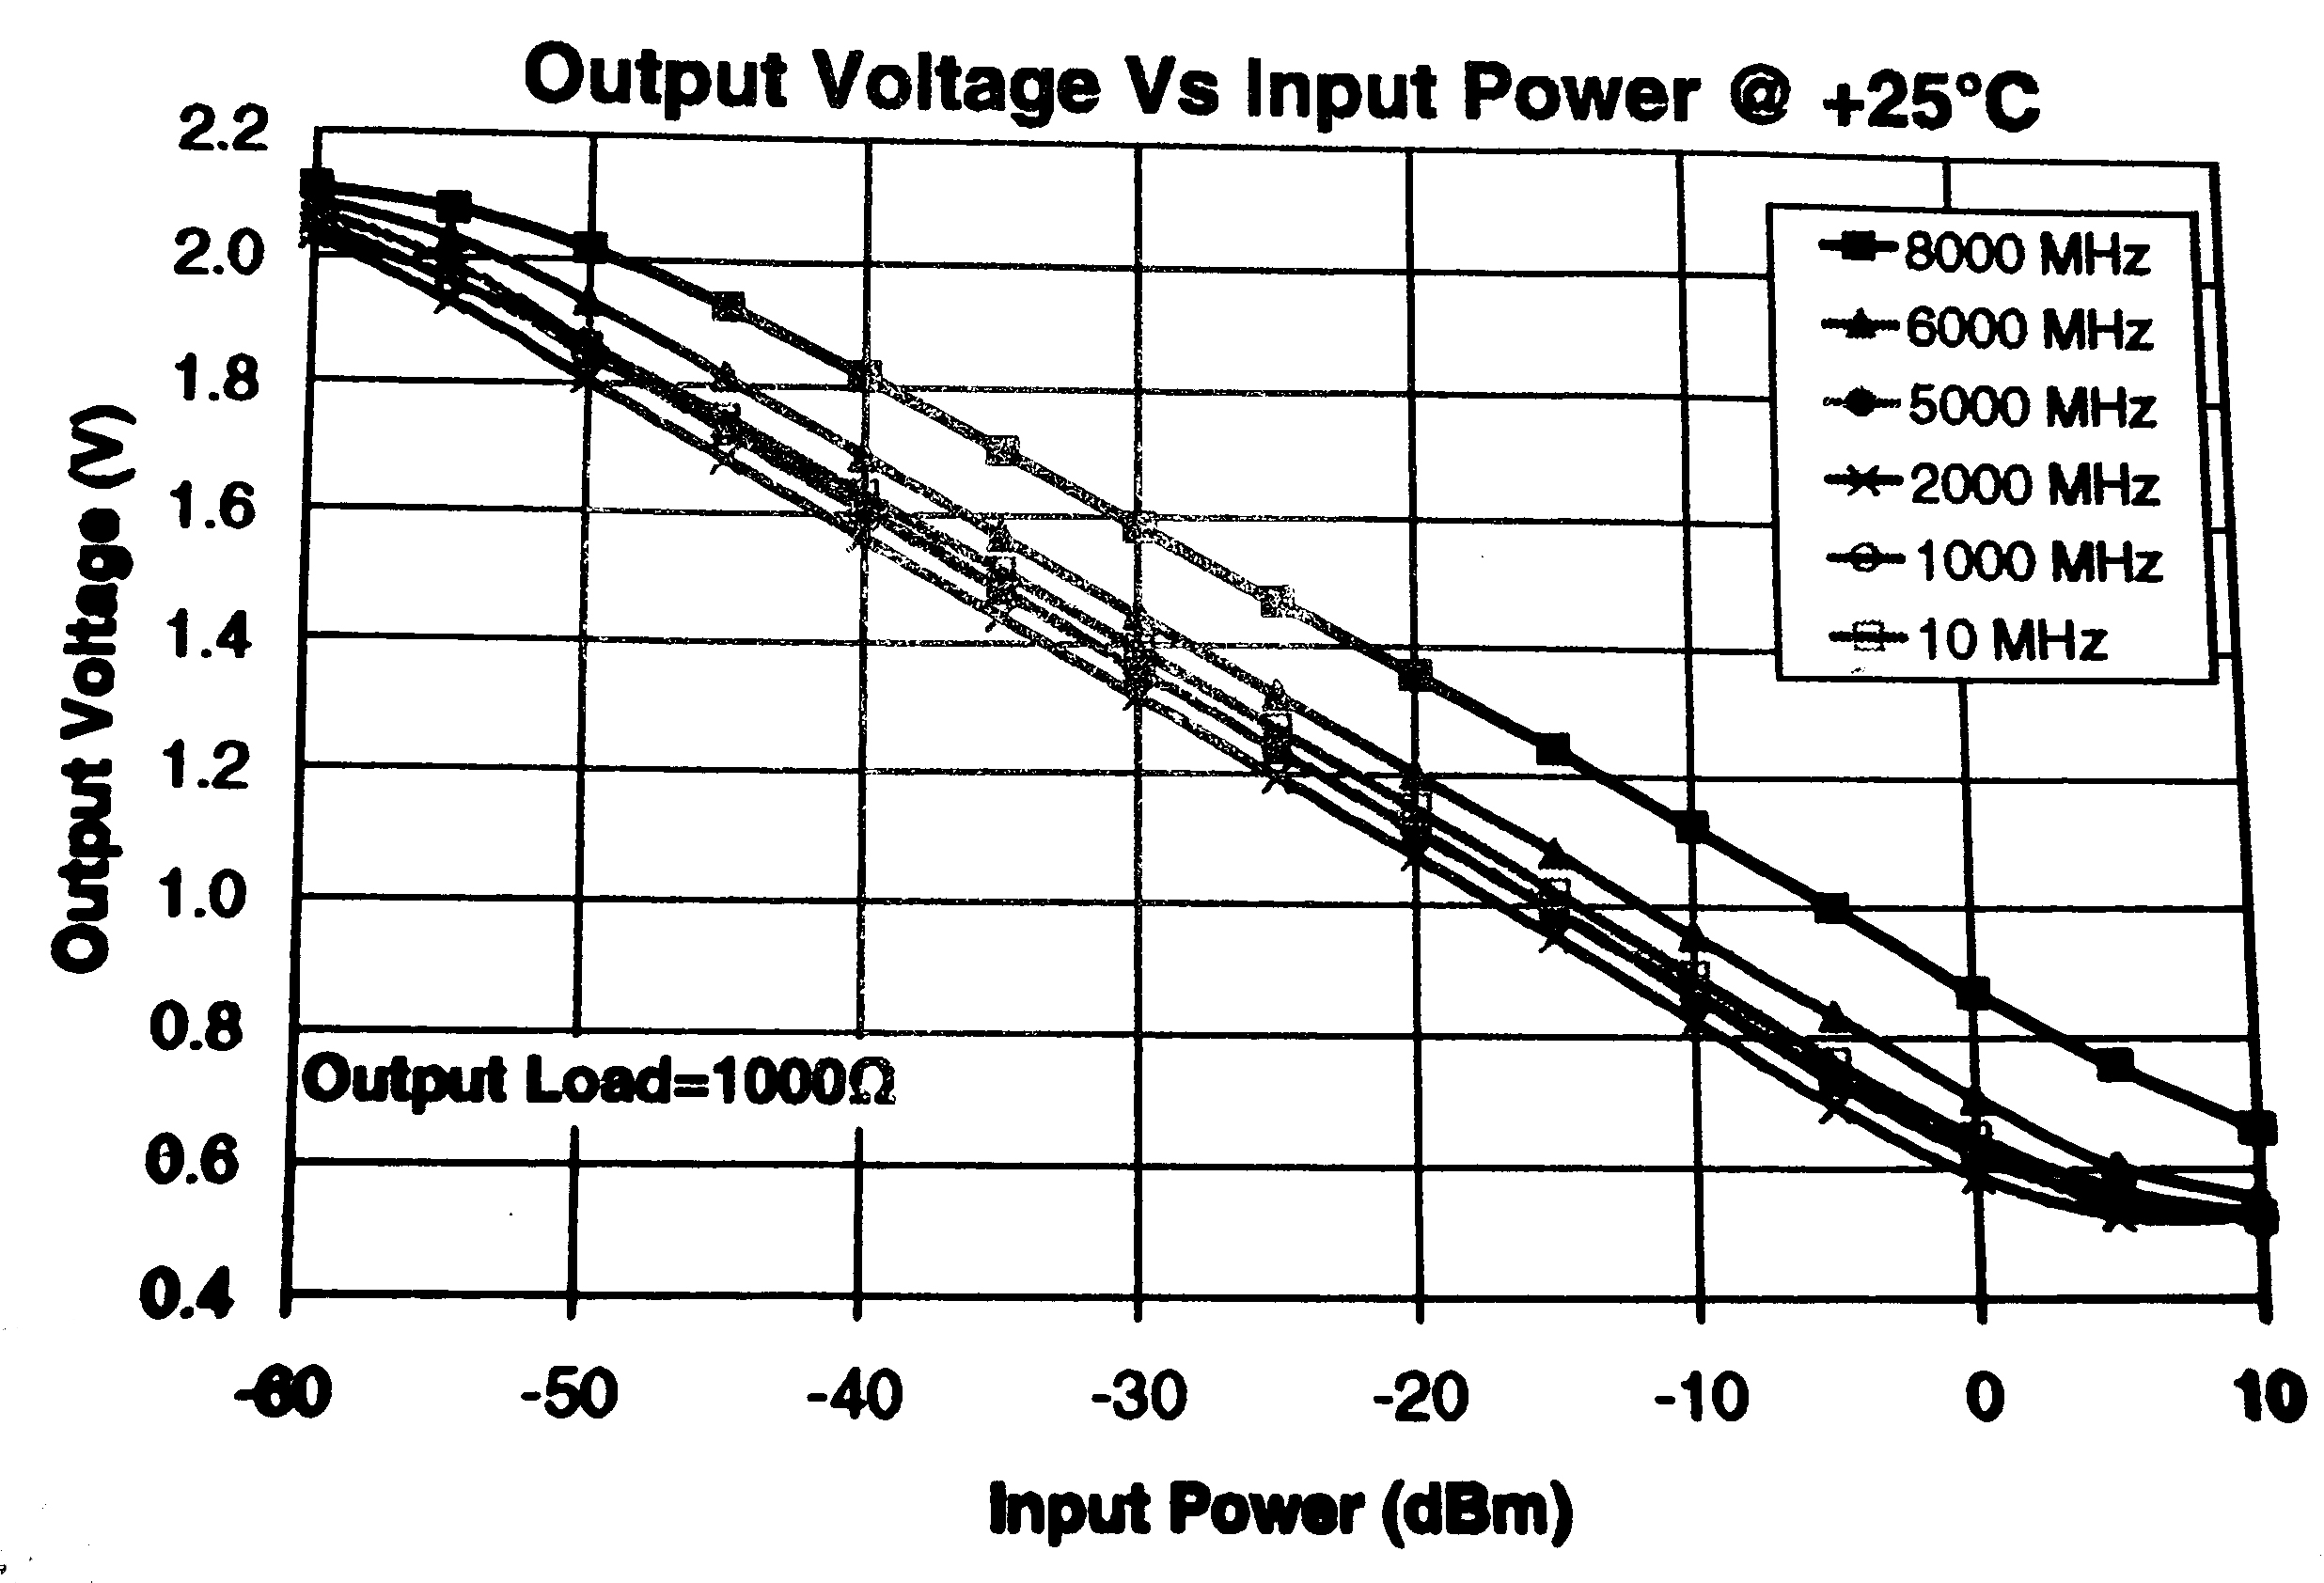
\includegraphics[scale=0.15]{figs/voltage_curve.JPG}
\caption{The convertor from voltage to power. }
\label{conv}
\end{center}
\end{figure}

 \begin{figure}[htb]
\begin{center}
 \includegraphics[scale=0.5]{code/errors.png}
\end{center}
\end{figure}
